\chapter{Evaluation}
\label{chap:evaluation}

\section{Energy Consumption}
\label{sec:energy-consumption}
    One of the main motivations for SNNs is their energy efficiency compared to ANNs on specialized hardware. Products like Loihi from Intel \cite{8259423} and TrueNorth from IBM \cite{7229264} have proved the potential of SNNs by utilizing the asynchronous communication via spikes. In the real-world scenario, one often uses accelerators like GPUs to train SNNs and deploy them on specialized hardware to achieve fast training and energy efficent inference. 

    Here we present an energy consumption model for the multi-bit spike train model and compare it with the 1-bit spike train model. We consider the unique properties of various hardware implementations and give the energy consumption of the multi-bit spike train model relative to the 1-bit spike train model. 

    \subsection{Training Energy Consumption on GPUs}
    \label{subsec:training_energy}
        On GPUs, low precision spikes are generally not very meaningful, as the hardware is not designed for such level mixed precision operations. Often the spikes are represented as 32-bit floating point numbers, which can be computed with the weights with the same precision. And the popular SNN frameworks like snnTorch and SpikingJelly do not utilize the sparsity of the spike trains. So here, the firing rate and the bit width of the spike train do not affect the energy consumption of the training phase. 
    
        The only factors that matter are the number of iterations required to reach a certain accuracy and the number of time steps that the network is simulated, assuming fixed network topology and batch size. 
    
        This allows us to create a simple, yet effective energy consumption model for the training phase on the GPUs. Let $T_i$ denote the number of time steps, $S_i$ denote the number of iterations required to reach a certain accuracy, and $E_{\text{train}-i}$ denote the energy consumption. Then we have:
        \begin{equation}
            E_{\text{train}-i} = T_i \cdot S_i \cdot c
        \end{equation}
        where as $c$ is a constant factor that depends on the hardware and the software used, however remains the same across different bit widths of the spike train. 
    
        As noticed in Section \ref{sec:convergence_accuracy}, one requires fewer iterations to reach a certain accuracy with the multi-bit spike train model. Here we focus on the energy consumption of the 2-bit spike train model, as it does not increase the firing rate as much as the other higher bit width models while still providing a significant improvement in convergence speed and accuracy. 

        Based on the results in Section \ref{fig:iterations_fixed_accuracy}, we can estimate the energy consumption of the 2-bit spike train model relative to the 1-bit spike train model directly by comparing the number of iterations required to reach a certain accuracy which is around $50.00\pm10.84\%$ in this case (see Figure \ref{fig:training_energy_gpu}). 
        \begin{figure}[!htpb]
            \centering
            \begin{subfigure}[H]{0.8\textwidth}
                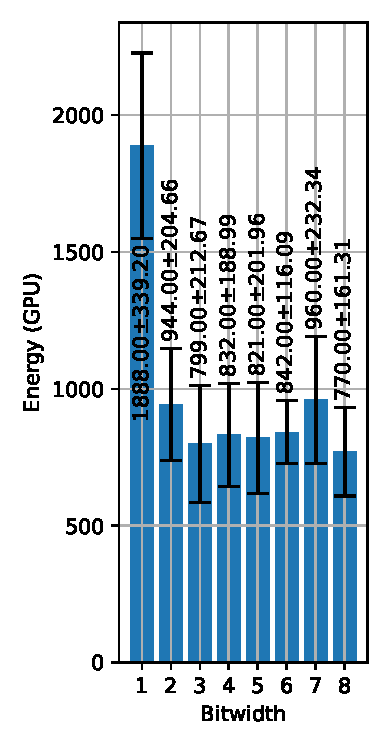
\includegraphics[width=\textwidth]{../standard/FashionMNIST/plots/fashionmnist_train_energy_gpu.pdf}
                \caption{Energy Consumption Estimation, Unit in Constant $c$}
            \end{subfigure}
            \hfill
            \begin{subfigure}[H]{0.8\textwidth}
                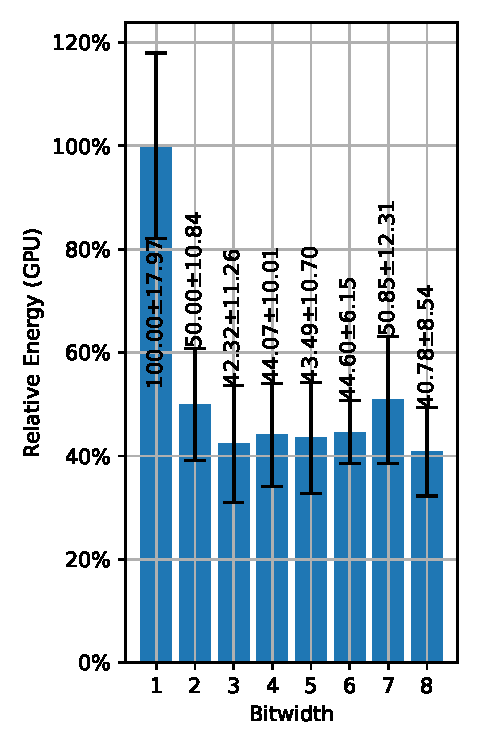
\includegraphics[width=\textwidth]{../standard/FashionMNIST/plots/fashionmnist_train_relative_energy_gpu.pdf}
                \caption{Normalized Energy Consumption Estimation Relative to 1-bit Spike Train Model}
            \end{subfigure}
            \caption{Training Energy Consumption Estimation on GPUs for Fashion MNIST Dataset}
            \label{fig:training_energy_gpu}
        \end{figure}

        See more in Appendix \ref{appendix:energy_gpu}.

    \subsection{Inference Energy Consumption on Neuromorphic Chips}
    \label{subsec:inference_energy}
        A widely adopted energy estimation model for neuromorphic chips is the following:
        \begin{equation}
            \label{eq:inference_energy_popular}
            E_{\text{inference}} = F \cdot fr \cdot E_{\text{AC}} \cdot T
        \end{equation}
        where $F$ is the number of floating point operations required to simulate the network, $fr$ is the firing rate of the neurons, $E_{\text{AC}}$ is the energy consumption of accumulation, and $T$ is the number of time steps. 
    
        It is however hard to evaluate the energy consumption of the multi-bit spike train model on neuromorphic chips like Loihi and TrueNorth, as they do not support multi-bit spikes natively. Although it may be possible to encode the multi-bit spikes into multiple spikes with different intensities, the energy consumption of such encoding is very expensive due to the high cost of the synchronization barrier between the time steps. 

        A viable option is to consider hardware like Intel Loihi 2 which supports graded spikes up to 32-bit precision. We consider the case of Intel Loihi 2 and make the following assumptions: 
        \begin{enumerate}
            \item There is no difference in the energy consumption for the number of bits used to encode the spikes.
            \item The energy consumption for a floating point operation is always $E_{\text{MAC}}$ (Multiply-Accumulate).
        \end{enumerate}
        Since the payload is not variable in this case, the energy consumption of the multi-bit spike train model is directly proportional to the firing rate given fixed maximum floating point operations and time steps. Analog as the equation \ref{eq:inference_energy_popular}, we have the following estimation for the $i$-bit spike train model:
        \begin{equation}
            E_{\text{inference}-i} = F \cdot fr_i \cdot E_{\text{MAC}} \cdot T_i
        \end{equation}
        We can estimate the energy consumption of the 2-bit spike train model relative to the 1-bit spike train model by comparing the firing rate of the neurons. As expected, the energy consumption of the multi-bit spike train model is higher than the 1-bit spike train model, as the firing rate of the neurons is higher (see Figure \ref{fig:inference_energy_nh}).
        \begin{figure}[!htpb]
            \centering
            \begin{subfigure}[H]{\textwidth}
                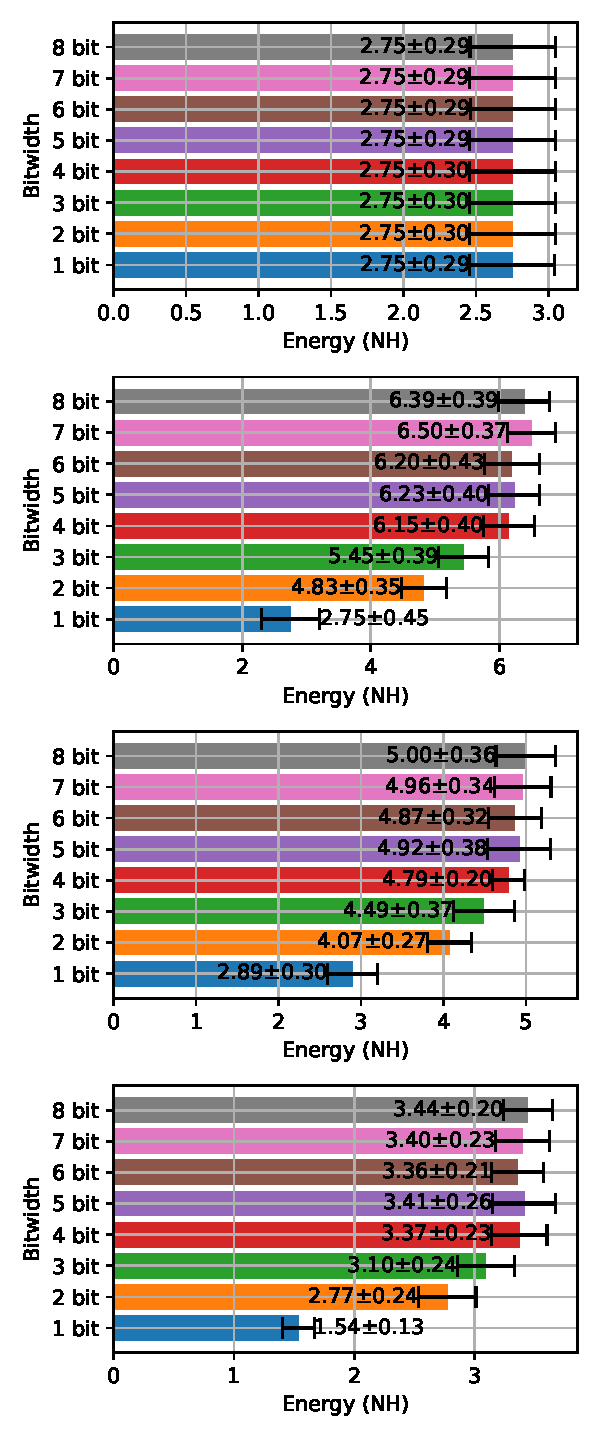
\includegraphics[width=\textwidth]{../standard/FashionMNIST/plots/fashionmnist_test_energy_nh.pdf}
                \caption{Energy Consumption Estimation, Unit in Parameters $F\cdot E_{\text{MAC}}$}
            \end{subfigure}
            \hfill
            \begin{subfigure}[H]{\textwidth}
                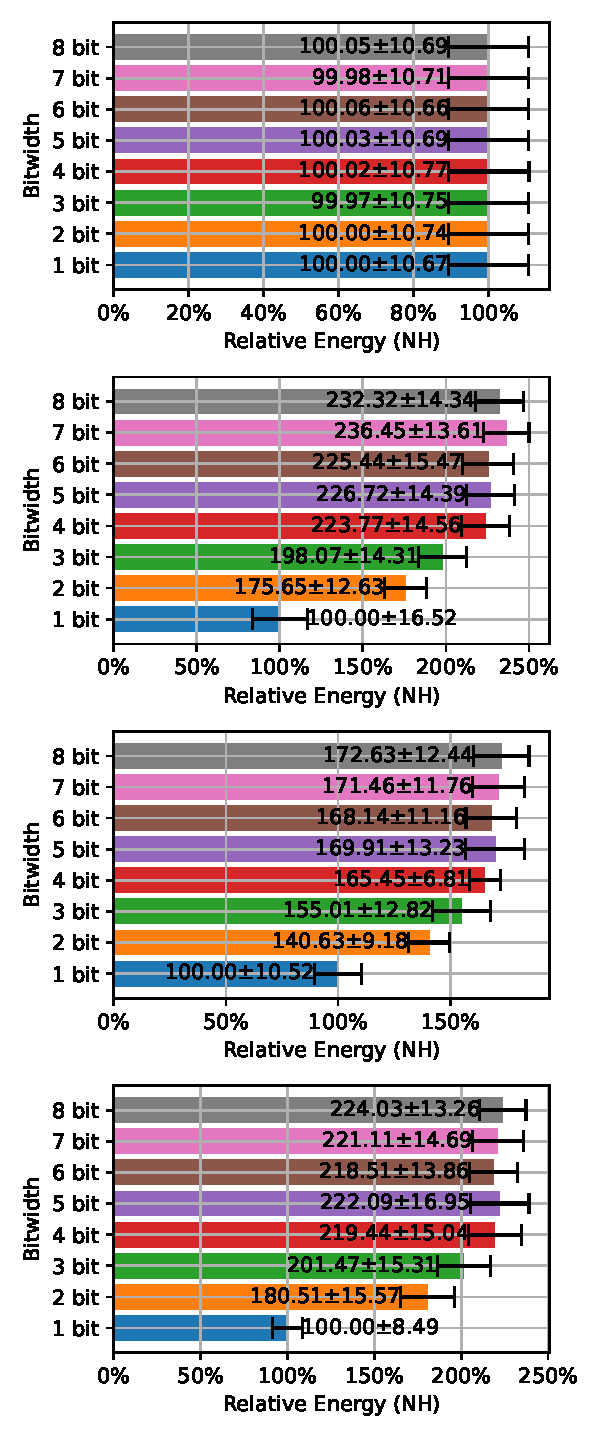
\includegraphics[width=\textwidth]{../standard/FashionMNIST/plots/fashionmnist_test_relative_energy_nh.pdf}
                \caption{Normalized Energy Consumption Estimation Relative to 1-bit Spike Train Model}
            \end{subfigure}
            \caption{Inference Energy Consumption Estimation on Intel Loihi 2 for Fashion MNIST Dataset}
            \label{fig:inference_energy_nh}
        \end{figure}

        See more in Appendix \ref{appendix:energy_neuromorphic}.
        %TODO: Add references to the analysis model

    \subsection{Tradeoffs}
        One can tell that the energy consumption of the multi-bit spike train model has no direct advantage over the 1-bit spike train model on neuromorphic chips, as the firing rate of the multi-bit spike train model tends to be higher than the 1-bit spike train model. Moreover, one can also argue that the energy consumption from $E_{\text{MAC}}$ is due to the graded spikes, which is not an issue with binary spikes. 

        We consider the energy consumption of the multi-bit spike train model in general as an opportunity to enable tradeoffs. If the inference is not the bottleneck of the application, then one can rely on the fast convergence speed of the multi-bit spike train model during training. If the inference is the bottleneck, then one can choose to train the multi-bit spike train model for longer time to achieve a firing rate that is comparable to the 1-bit spike train model (see Figure \ref{fig:inference_energy_nh_firerate}). Such tradeoffs are not possible with the 1-bit spike train model. 
        \begin{figure}[!htpb]
            \centering
            \begin{subfigure}[H]{0.48\textwidth}
                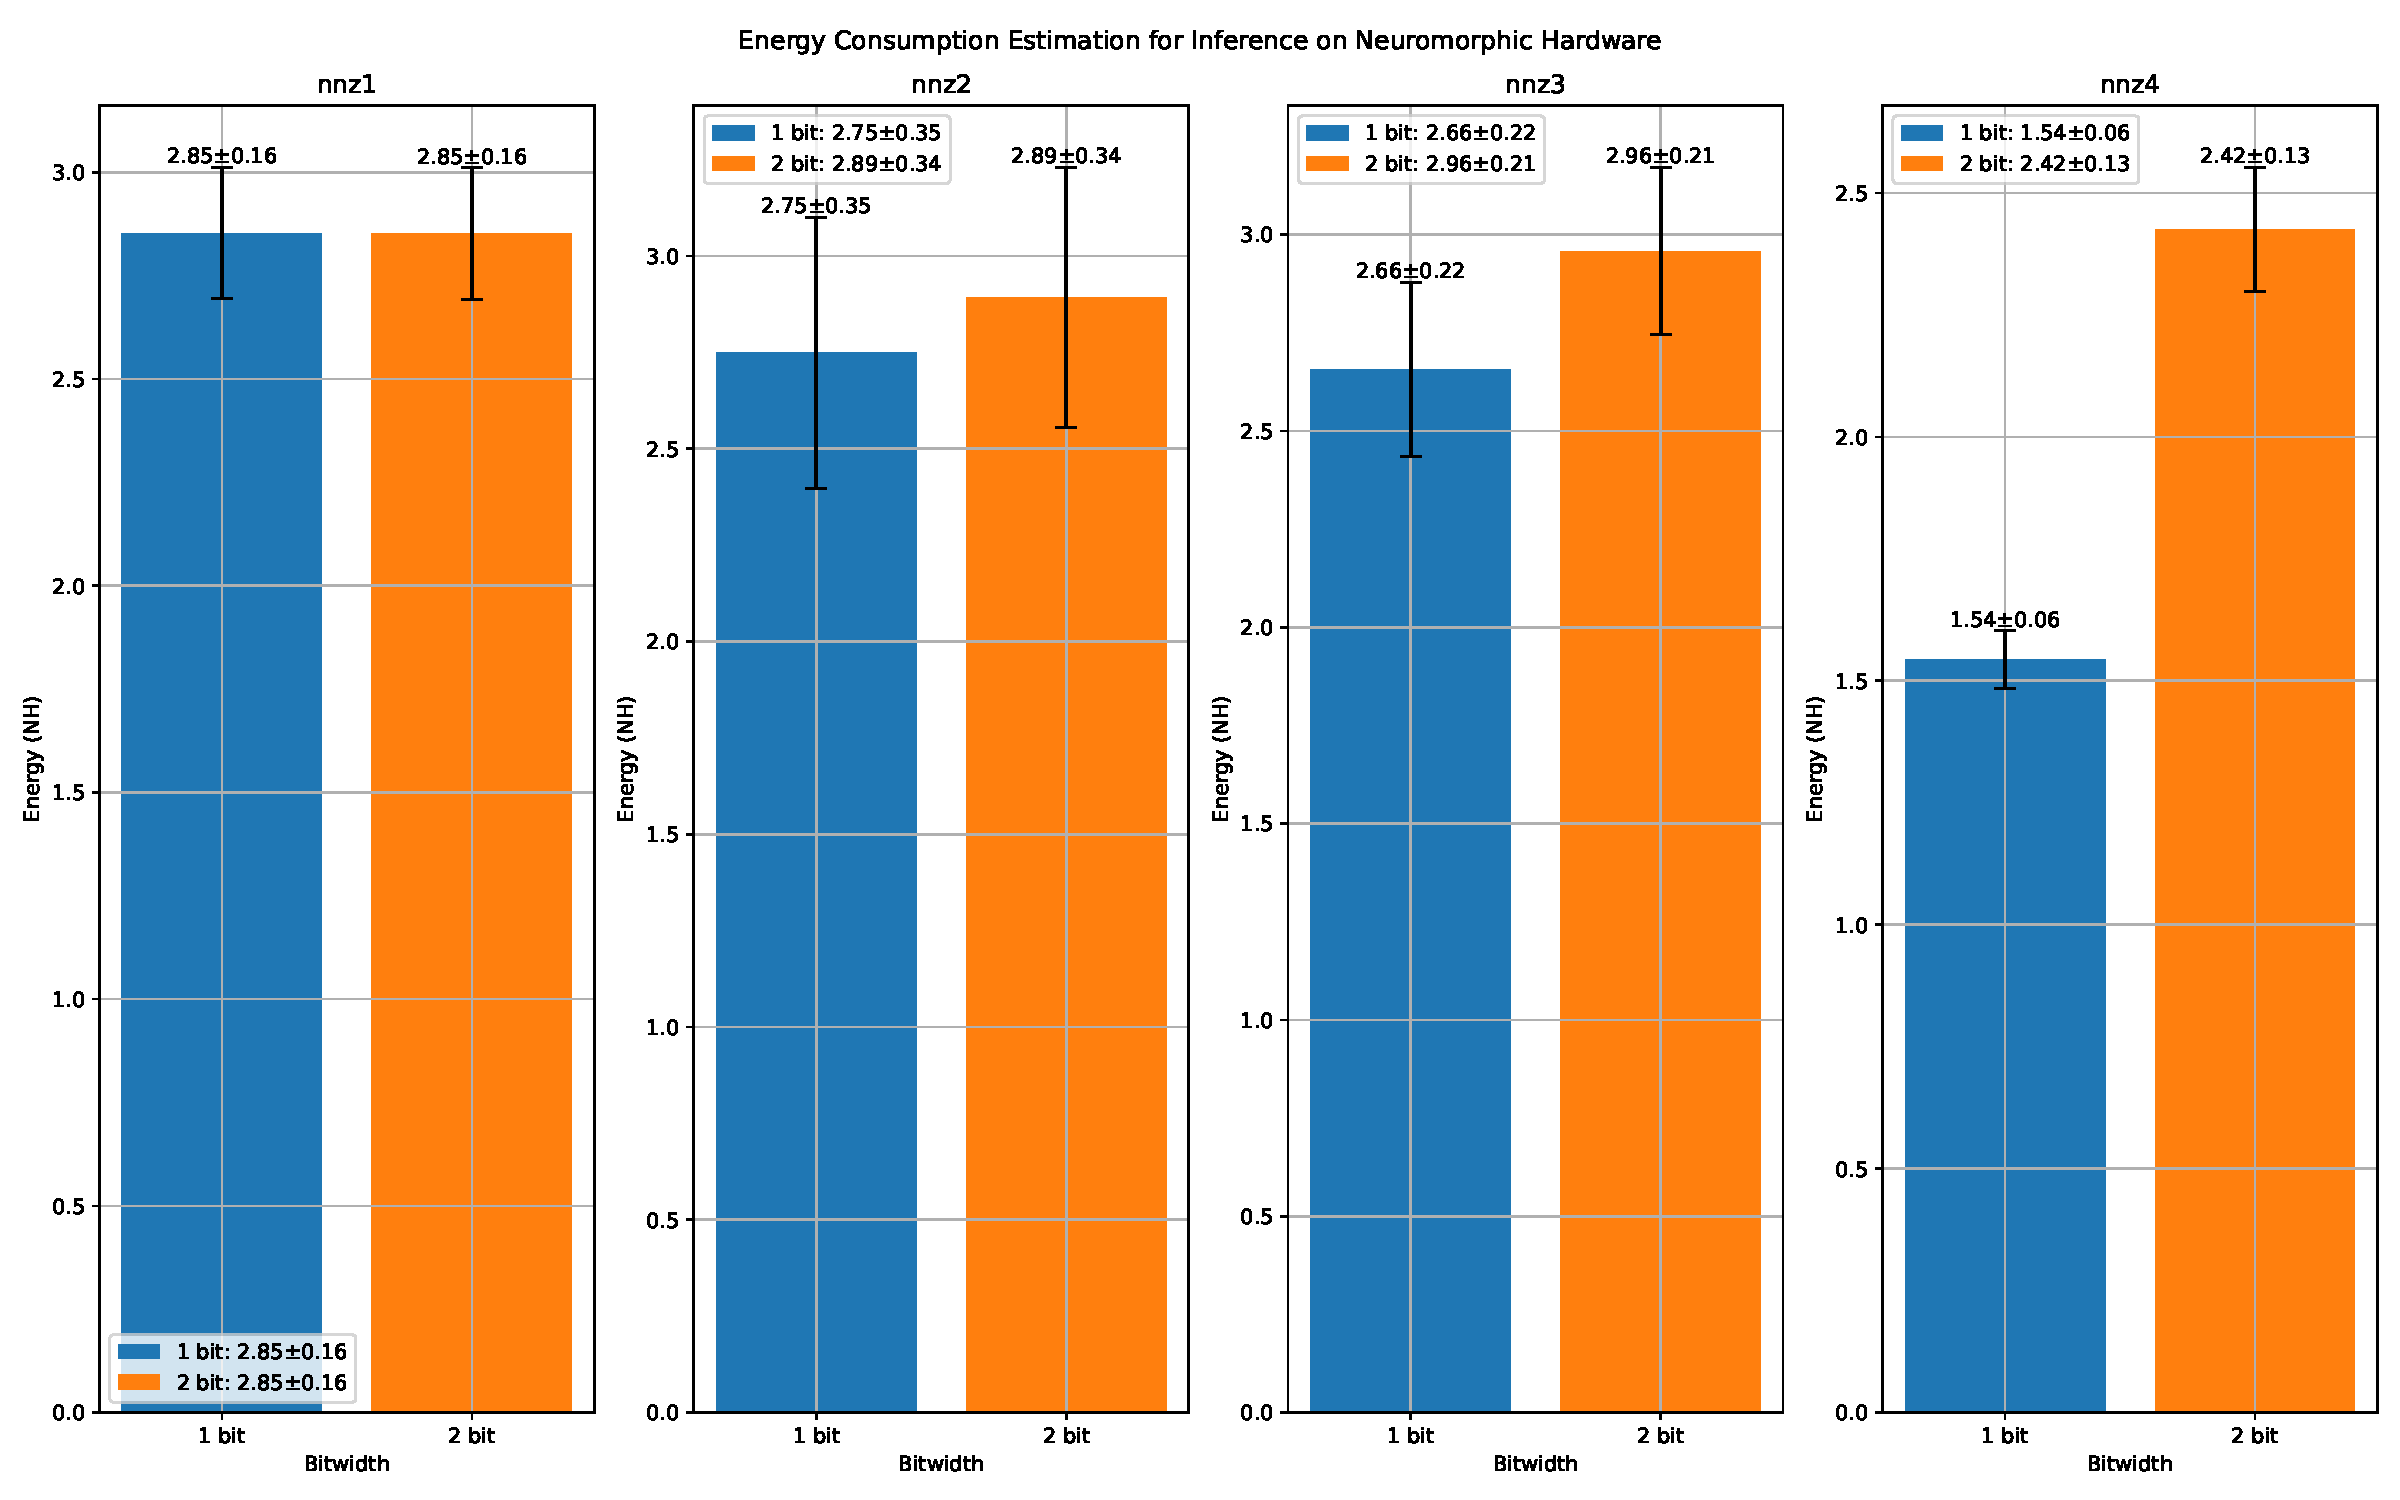
\includegraphics[width=\textwidth]{../firerate/FashionMNIST/plots/fashionmnist_test_energy_nh.pdf}
                \caption{Energy Consumption Estimation, Unit in Parameters $F\cdot E_{\text{MAC}}$}
            \end{subfigure}
            \hfill
            \begin{subfigure}[H]{0.48\textwidth}
                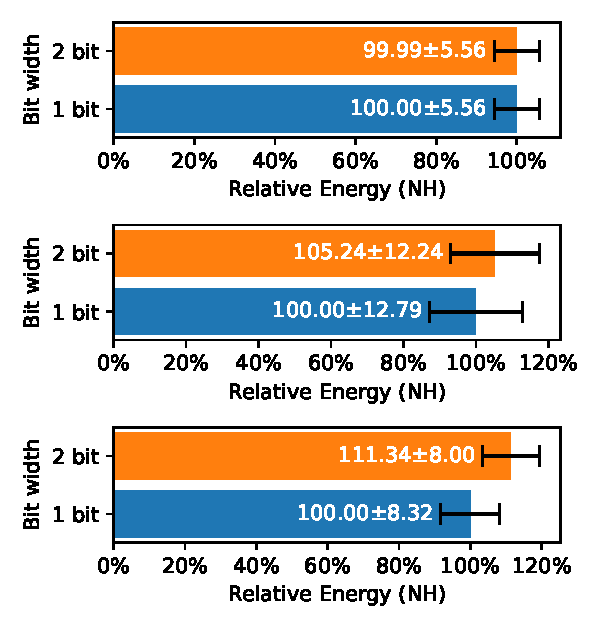
\includegraphics[width=\textwidth]{../firerate/FashionMNIST/plots/fashionmnist_test_relative_energy_nh.pdf}
                \caption{Normalized Energy Consumption Estimation Relative to 1-bit Spike Train Model}
            \end{subfigure}
            \caption{Inference Energy Consumption Estimation on Intel Loihi 2 for Fashion MNIST Dataset with 50 Training Epochs}
            \label{fig:inference_energy_nh_firerate}
        \end{figure}

        And more interestingly, if one is satisfied with the accuracy of the 1-bit spike train model, then one can choose to train the multi-bit spike train model for fewer time steps. This can enable higher efficiency in both training and inference. 

        We take again the example of Fashion MNIST dataset, while $T=10$ is a good choice for both the 1-bit and 2-bit spike train model, we can reduce the time steps to $T=4$ for the 2-bit spike train model and still achieve a comparable accuracy (see \ref{fig:inference_energy_nh_timesteps}). 
        \begin{figure}[!htpb]
            \centering
            \begin{subfigure}[H]{0.48\textwidth}
                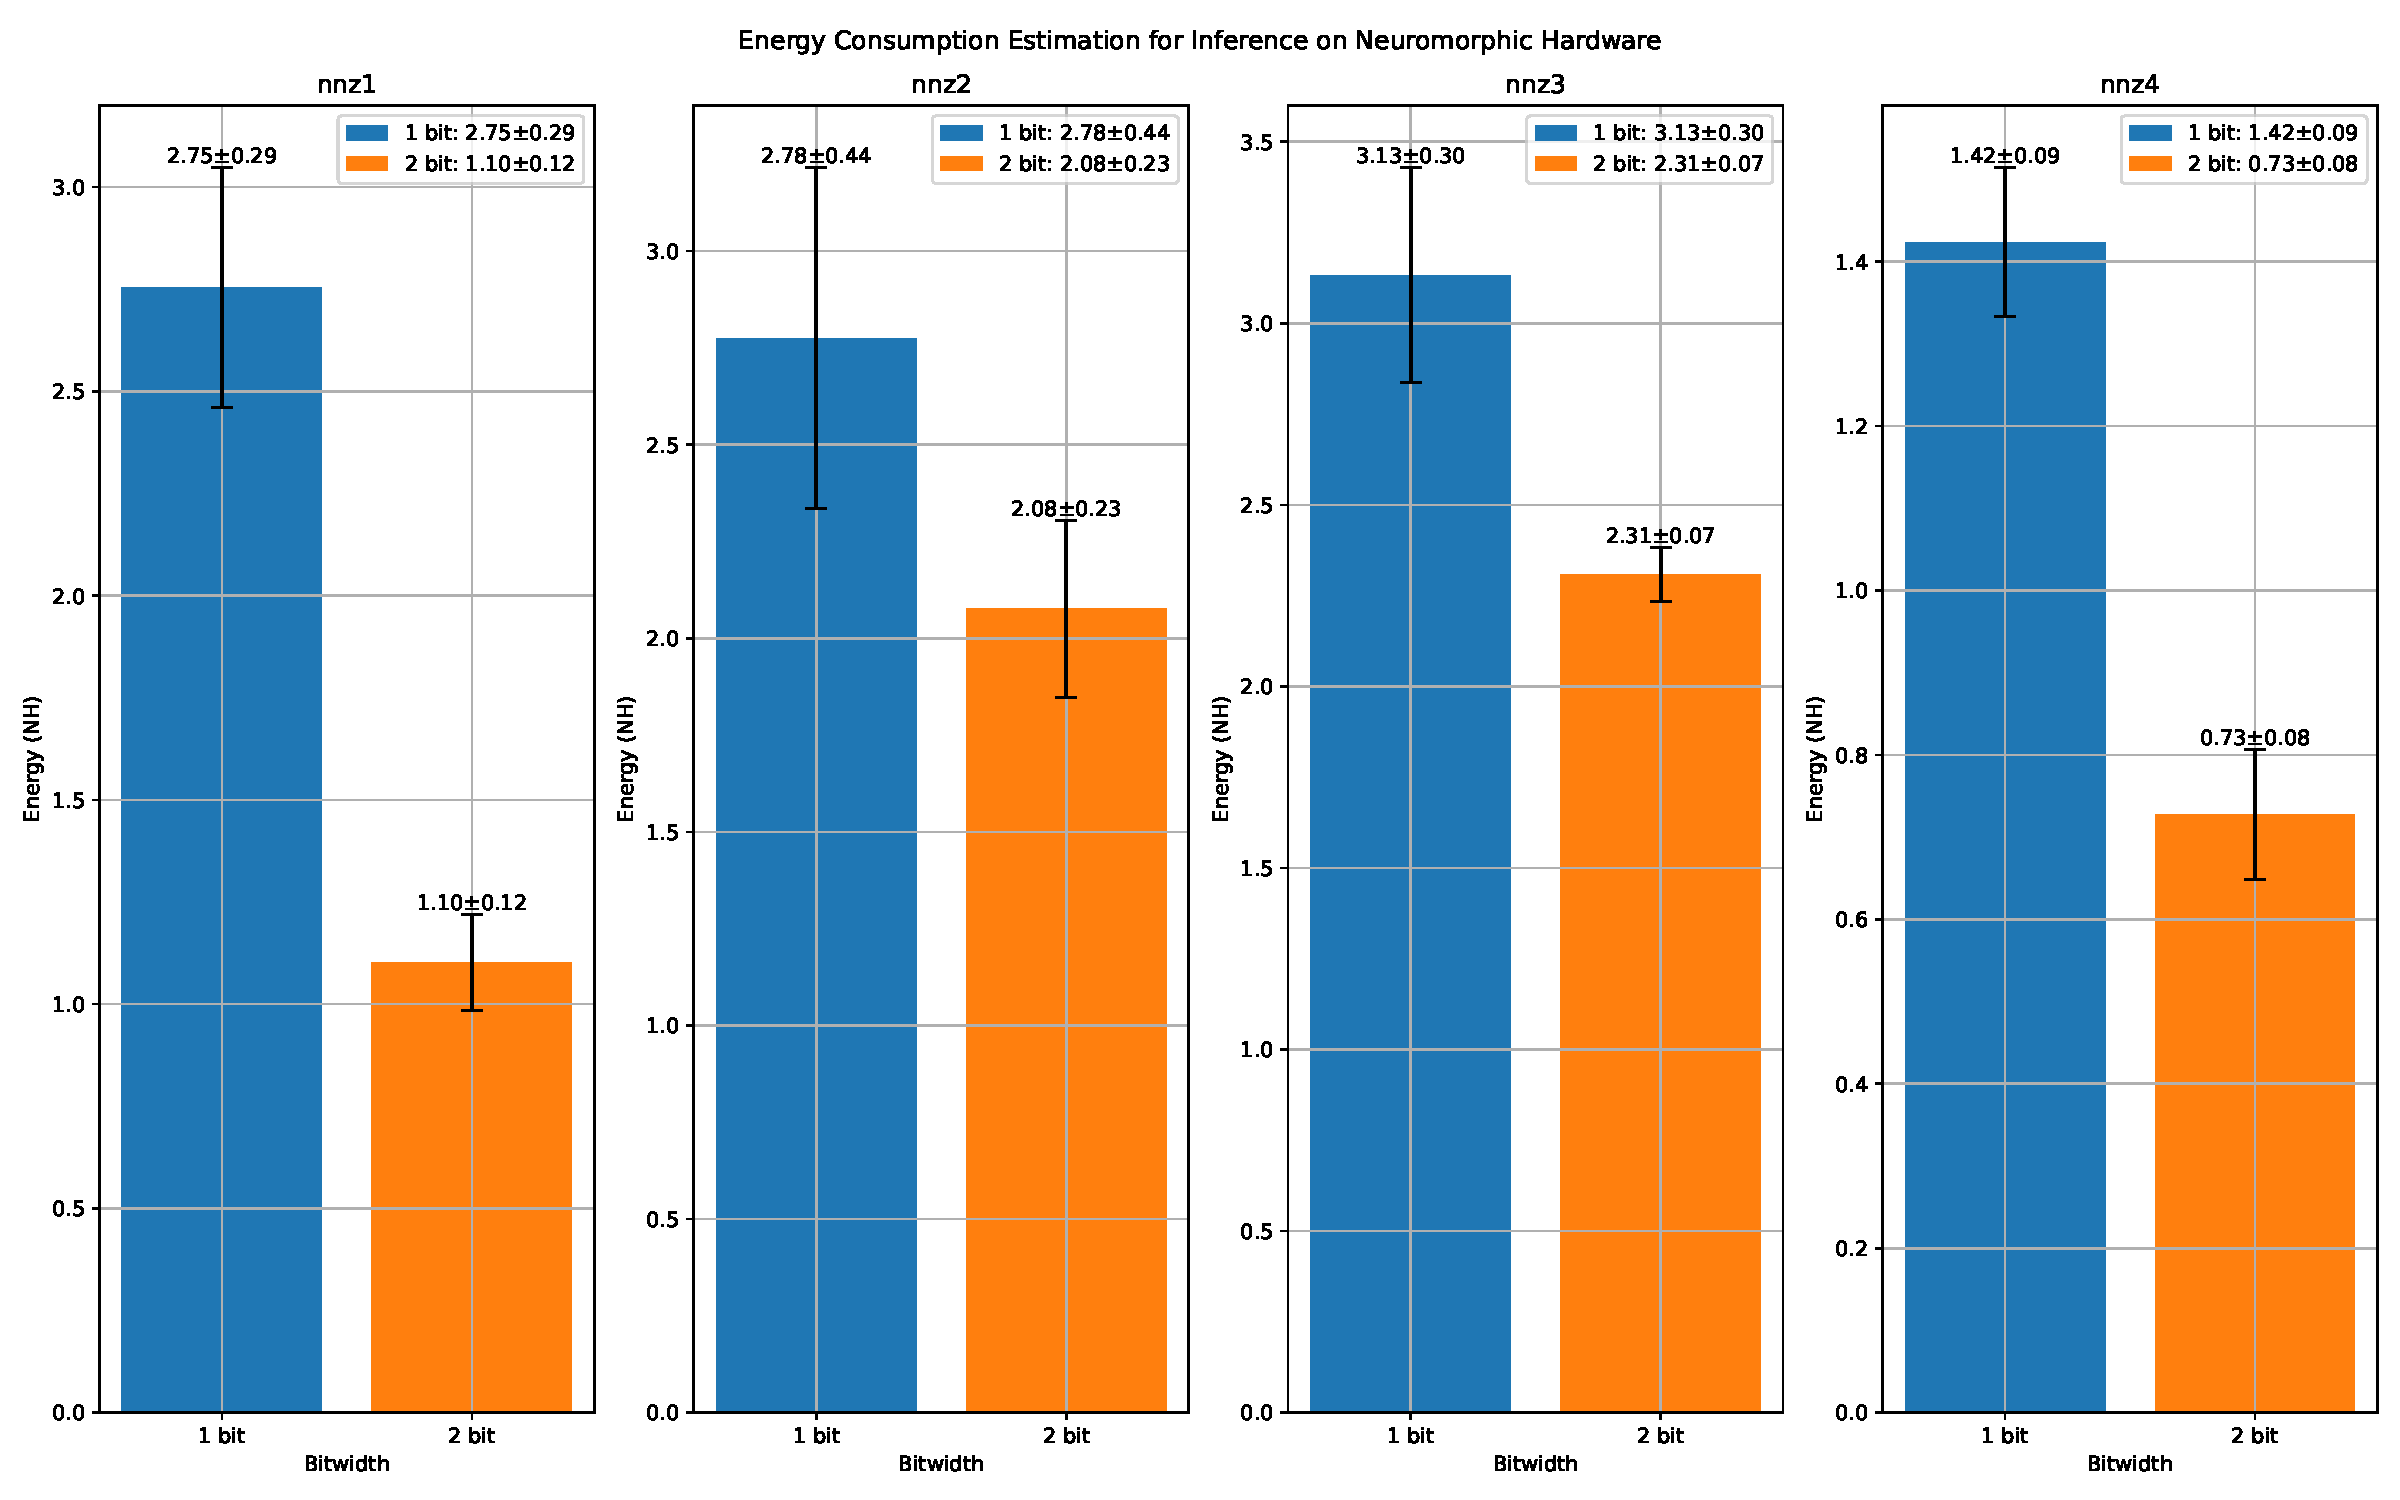
\includegraphics[width=\textwidth]{../timesteps/FashionMNIST/plots/fashionmnist_test_energy_nh.pdf}
                \caption{Energy Consumption Estimation, Unit in Parameters $F\cdot E_{\text{MAC}}$}
            \end{subfigure}
            \hfill
            \begin{subfigure}[H]{0.48\textwidth}
                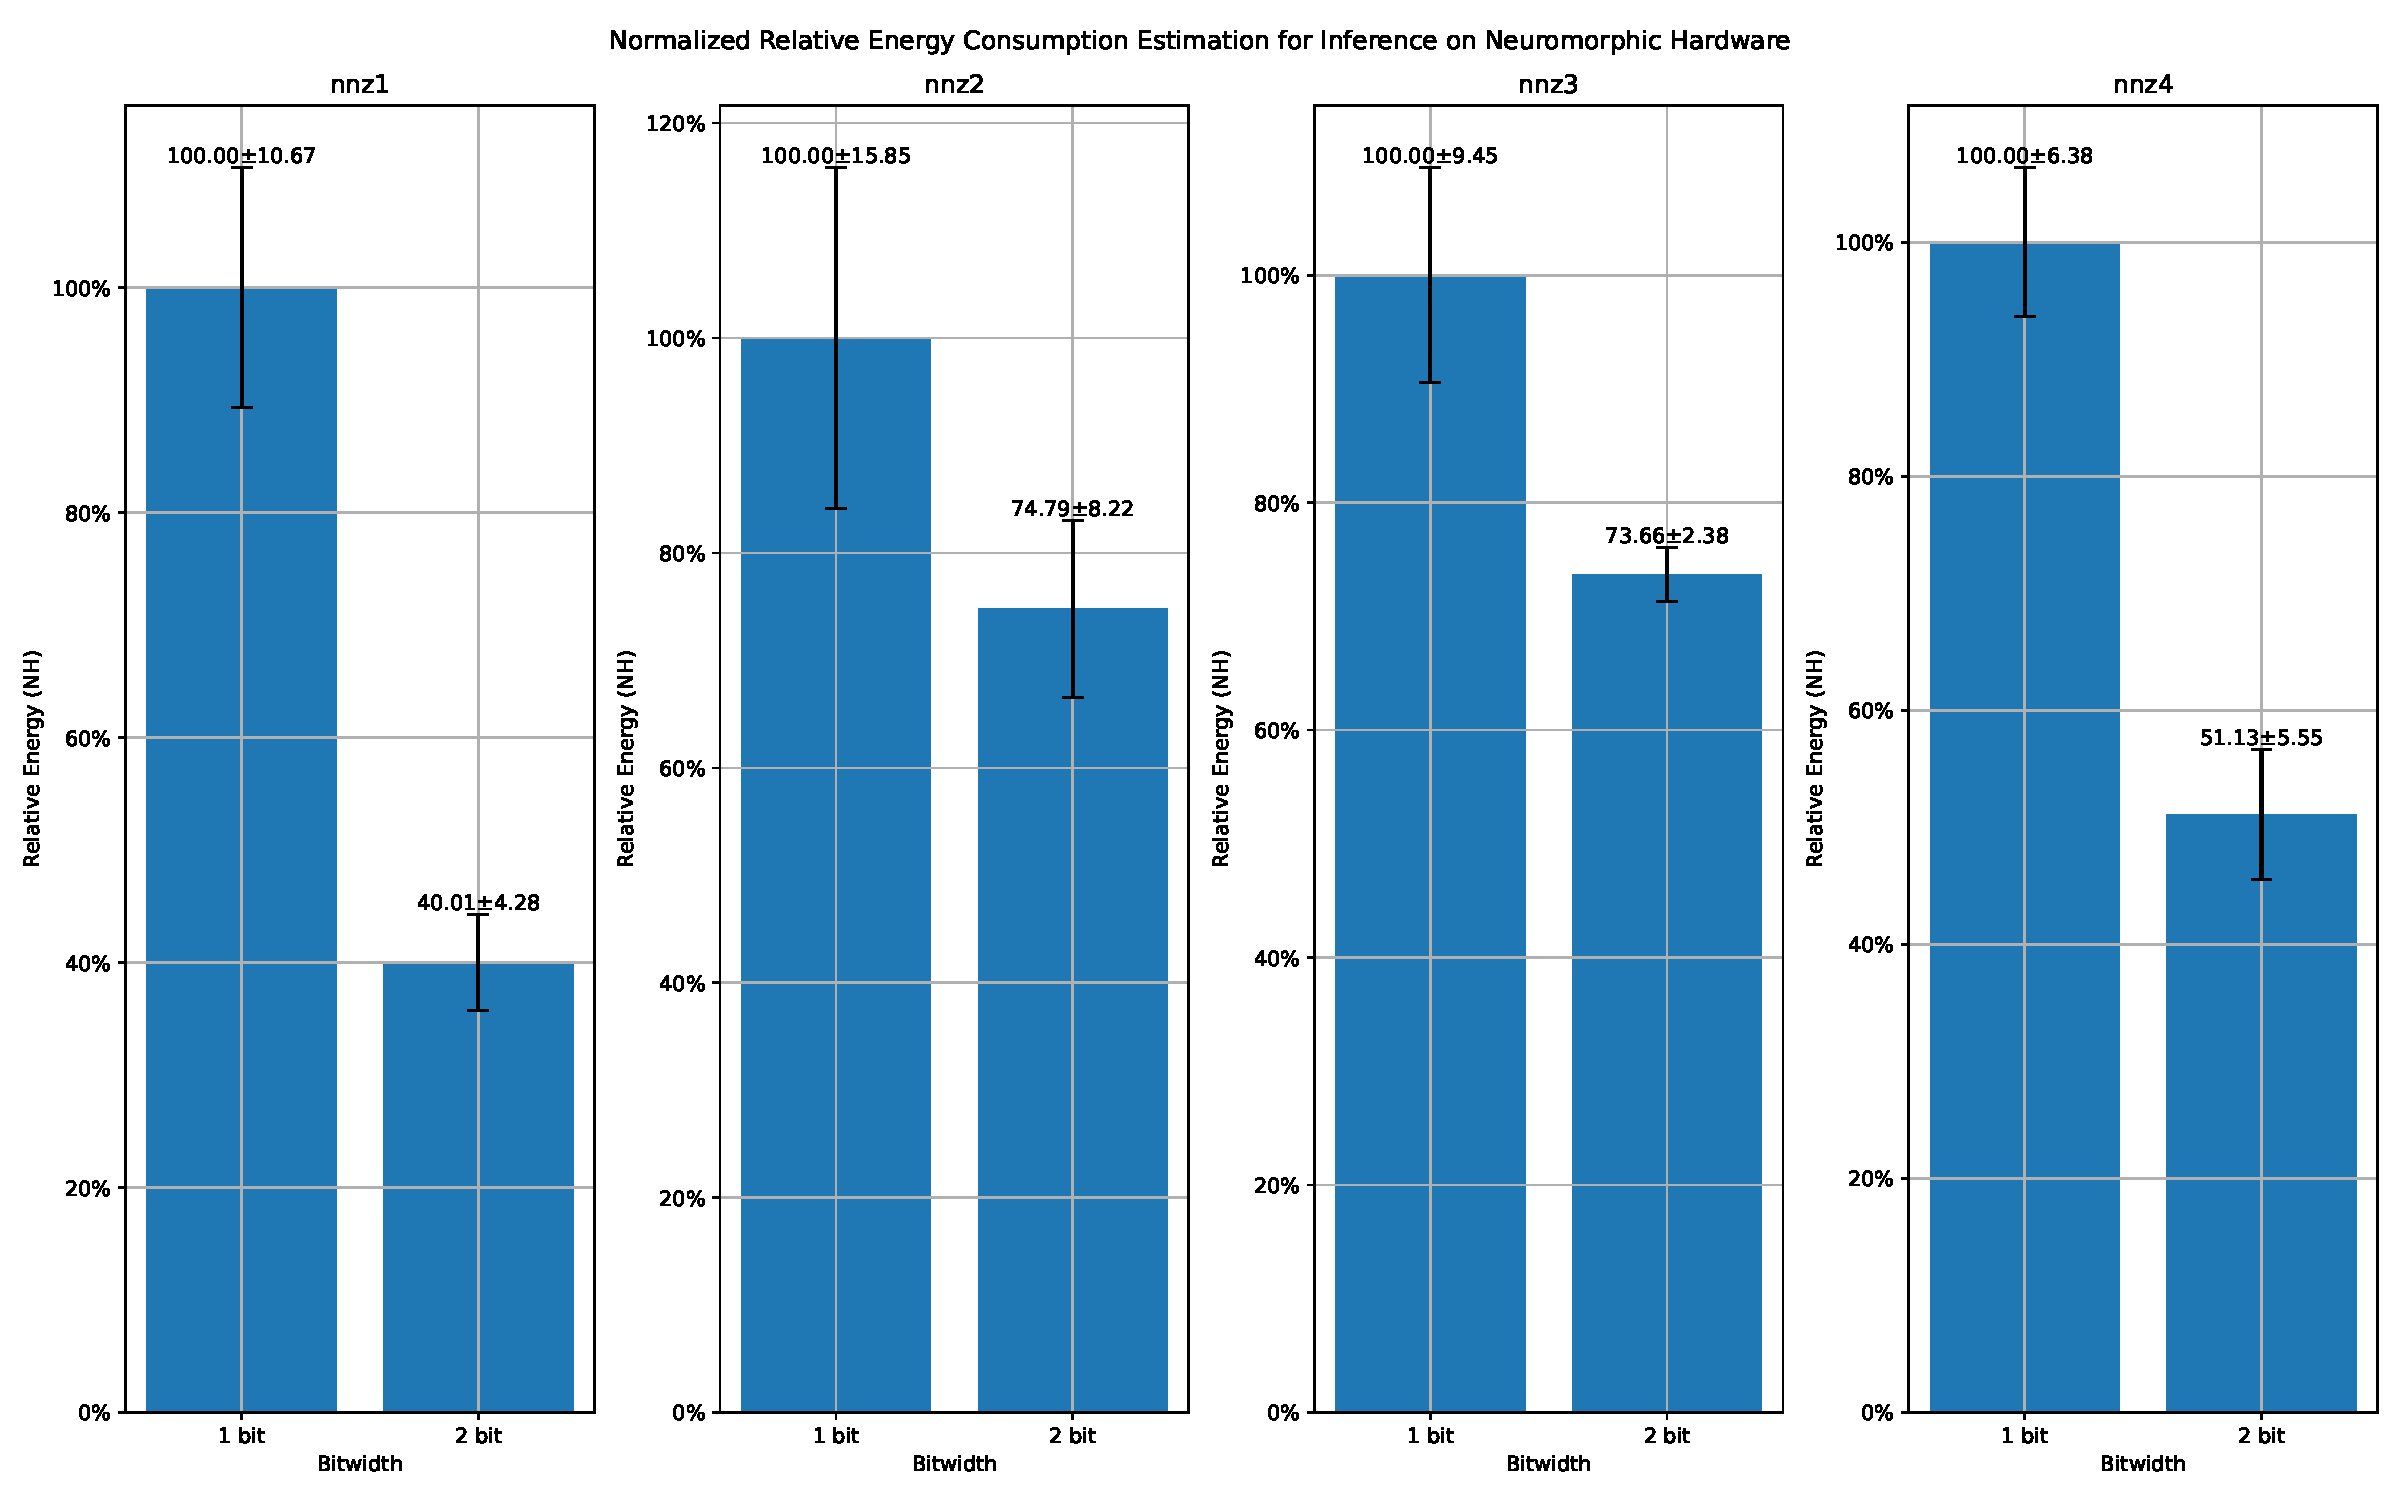
\includegraphics[width=\textwidth]{../timesteps/FashionMNIST/plots/fashionmnist_test_relative_energy_nh.pdf}
                \caption{Normalized Energy Consumption Estimation Relative to 1-bit Spike Train Model}
            \end{subfigure}
            \hfill
            \begin{subfigure}[H]{\textwidth}
                \centering
                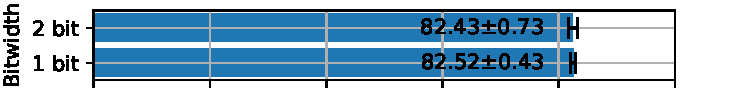
\includegraphics[width=\textwidth]{../timesteps/FashionMNIST/plots/fashionmnist_final_acc.pdf}
                \caption{Accuracy Comparison}
            \end{subfigure}
            \caption{Inference Energy Consumption Estimation on Intel Loihi 2 and Test Accuracy for Fashion MNIST Dataset with 10 Time Steps for 1-bit Spike Train Model and 4 Time Steps for 2-bit Spike Train Model}
            \label{fig:inference_energy_nh_timesteps}
        \end{figure}
        
        See more in Appendix \ref{appendix:energy_tradeoff}.

        This can lead to a significant reduction in the energy consumption. It may not be reflected as a direct advantage in the energy consumption model mentioned above \ref{subsec:inference_energy}, but in practice, it should bring significant benefits, as most of the neuromorphic chips are designed to utilize the asynchronous communication via spikes, so they do not have a central clock system to synchronize the time steps very efficiently, and the cost for the synchronization barrier is very high. As reference, the latency per tile hop on Intel Loihi is at most around 6.5 ns where as the latency for the synchronization barrier is from 113-465 ns. 

\section{Performance}
\label{sec:performance}
    In the section \ref{subsec:training_energy}, we claim that the energy consumption on the GPUs are not affected by the firing rate and the bit width of the spike train in theory. However, in practice, with the increase of the bit width of the spike train, the training process slows down. This can be caused by the inefficient implementation of the multi-bit spike train model and the low level optimization on operations of sparse matrix multiplication. 

    There is sufficient room for improvement, e.g. by utilizing the sparsity of the spike trains or completely switching to the vectorized model instead of the temporal model instead, which is shown to be more efficient with learning algorithms like SLAYER and EXODUS. 
